\documentclass[12pt]{beamer}\usepackage[]{graphicx}\usepackage[]{color}
%% maxwidth is the original width if it is less than linewidth
%% otherwise use linewidth (to make sure the graphics do not exceed the margin)
\makeatletter
\def\maxwidth{ %
  \ifdim\Gin@nat@width>\linewidth
    \linewidth
  \else
    \Gin@nat@width
  \fi
}
\makeatother

\definecolor{fgcolor}{rgb}{0.345, 0.345, 0.345}
\newcommand{\hlnum}[1]{\textcolor[rgb]{0.686,0.059,0.569}{#1}}%
\newcommand{\hlstr}[1]{\textcolor[rgb]{0.192,0.494,0.8}{#1}}%
\newcommand{\hlcom}[1]{\textcolor[rgb]{0.678,0.584,0.686}{\textit{#1}}}%
\newcommand{\hlopt}[1]{\textcolor[rgb]{0,0,0}{#1}}%
\newcommand{\hlstd}[1]{\textcolor[rgb]{0.345,0.345,0.345}{#1}}%
\newcommand{\hlkwa}[1]{\textcolor[rgb]{0.161,0.373,0.58}{\textbf{#1}}}%
\newcommand{\hlkwb}[1]{\textcolor[rgb]{0.69,0.353,0.396}{#1}}%
\newcommand{\hlkwc}[1]{\textcolor[rgb]{0.333,0.667,0.333}{#1}}%
\newcommand{\hlkwd}[1]{\textcolor[rgb]{0.737,0.353,0.396}{\textbf{#1}}}%
\let\hlipl\hlkwb

\usepackage{framed}
\makeatletter
\newenvironment{kframe}{%
 \def\at@end@of@kframe{}%
 \ifinner\ifhmode%
  \def\at@end@of@kframe{\end{minipage}}%
  \begin{minipage}{\columnwidth}%
 \fi\fi%
 \def\FrameCommand##1{\hskip\@totalleftmargin \hskip-\fboxsep
 \colorbox{shadecolor}{##1}\hskip-\fboxsep
     % There is no \\@totalrightmargin, so:
     \hskip-\linewidth \hskip-\@totalleftmargin \hskip\columnwidth}%
 \MakeFramed {\advance\hsize-\width
   \@totalleftmargin\z@ \linewidth\hsize
   \@setminipage}}%
 {\par\unskip\endMakeFramed%
 \at@end@of@kframe}
\makeatother

\definecolor{shadecolor}{rgb}{.97, .97, .97}
\definecolor{messagecolor}{rgb}{0, 0, 0}
\definecolor{warningcolor}{rgb}{1, 0, 1}
\definecolor{errorcolor}{rgb}{1, 0, 0}
\newenvironment{knitrout}{}{} % an empty environment to be redefined in TeX

\usepackage{alltt}
\usepackage{graphicx}
\usepackage{tikz}
\setbeameroption{hide notes}
\setbeamertemplate{note page}[plain]
\usepackage{listings}

% get rid of junk
\usetheme{default}
\usefonttheme[onlymath]{serif}
\beamertemplatenavigationsymbolsempty
\hypersetup{pdfpagemode=UseNone} % don't show bookmarks on initial view

% named colors
\definecolor{offwhite}{RGB}{255,250,240}
\definecolor{gray}{RGB}{155,155,155}

\ifx\notescolors\undefined % slides

  \definecolor{foreground}{RGB}{80,80,80}
  \definecolor{background}{RGB}{255,255,255}
  \definecolor{title}{RGB}{255,199,0}
  \definecolor{subtitle}{RGB}{89,132,212}
  \definecolor{hilit}{RGB}{248,117,79}
  \definecolor{vhilit}{RGB}{255,111,207}
  \definecolor{lolit}{RGB}{200,200,200}
  \definecolor{lit}{RGB}{255,199,0}
  \definecolor{mdlit}{RGB}{89,132,212}
  \definecolor{link}{RGB}{248,117,79}

\else % notes
  \definecolor{background}{RGB}{255,255,255}
  \definecolor{foreground}{RGB}{24,24,24}
  \definecolor{title}{RGB}{27,94,134}
  \definecolor{subtitle}{RGB}{22,175,124}
  \definecolor{hilit}{RGB}{122,0,128}
  \definecolor{vhilit}{RGB}{255,0,128}
  \definecolor{lolit}{RGB}{95,95,95}
\fi
\definecolor{nhilit}{RGB}{128,0,128}  % hilit color in notes
\definecolor{nvhilit}{RGB}{255,0,128} % vhilit for notes

\newcommand{\hilit}{\color{hilit}}
\newcommand{\vhilit}{\color{vhilit}}
\newcommand{\nhilit}{\color{nhilit}}
\newcommand{\nvhilit}{\color{nvhilit}}
\newcommand{\lit}{\color{lit}}
\newcommand{\mdlit}{\color{mdlit}}
\newcommand{\lolit}{\color{lolit}}

% use those colors
\setbeamercolor{titlelike}{fg=title}
\setbeamercolor{subtitle}{fg=subtitle}
\setbeamercolor{frametitle}{fg=gray}
\setbeamercolor{structure}{fg=subtitle}
\setbeamercolor{institute}{fg=lolit}
\setbeamercolor{normal text}{fg=foreground,bg=background}
%\setbeamercolor{item}{fg=foreground} % color of bullets
%\setbeamercolor{subitem}{fg=hilit}
%\setbeamercolor{itemize/enumerate subbody}{fg=lolit}
\setbeamertemplate{itemize subitem}{{\textendash}}
\setbeamerfont{itemize/enumerate subbody}{size=\footnotesize}
\setbeamerfont{itemize/enumerate subitem}{size=\footnotesize}

% center title of slides
\setbeamertemplate{blocks}[rounded]
\setbeamertemplate{frametitle}[default][center]
% margins
\setbeamersize{text margin left=25pt,text margin right=25pt}

% page number
\setbeamertemplate{footline}{%
    \raisebox{5pt}{\makebox[\paperwidth]{\hfill\makebox[20pt]{\lolit
          \scriptsize\insertframenumber}}}\hspace*{5pt}}

% add a bit of space at the top of the notes page
\addtobeamertemplate{note page}{\setlength{\parskip}{12pt}}

% default link color
\hypersetup{colorlinks, urlcolor={link}}

\ifx\notescolors\undefined % slides
  % set up listing environment
  \lstset{language=bash,
          basicstyle=\ttfamily\scriptsize,
          frame=single,
          commentstyle=,
          backgroundcolor=\color{darkgray},
          showspaces=false,
          showstringspaces=false
          }
\else % notes
  \lstset{language=bash,
          basicstyle=\ttfamily\scriptsize,
          frame=single,
          commentstyle=,
          backgroundcolor=\color{offwhite},
          showspaces=false,
          showstringspaces=false
          }
\fi

% a few macros
\newcommand{\code}[1]{\texttt{#1}}
\newcommand{\hicode}[1]{{\hilit \texttt{#1}}}
\newcommand{\bb}[1]{\begin{block}{#1}}
\newcommand{\eb}{\end{block}}
\newcommand{\bi}{\begin{itemize}}
%\newcommand{\bbi}{\vspace{24pt} \begin{itemize} \itemsep8pt}
\newcommand{\bbi}{\vspace{4pt} \begin{itemize} \itemsep8pt}
\newcommand{\ei}{\end{itemize}}
\newcommand{\bv}{\begin{verbatim}}
\newcommand{\ev}{\end{verbatim}}
\newcommand{\ig}{\includegraphics}
\newcommand{\subt}[1]{{\footnotesize \color{subtitle} {#1}}}
\newcommand{\ttsm}{\tt \small}
\newcommand{\ttfn}{\tt \footnotesize}
\newcommand{\figh}[2]{\centerline{\includegraphics[height=#2\textheight]{#1}}}
\newcommand{\figw}[2]{\centerline{\includegraphics[width=#2\textwidth]{#1}}}



%------------------------------------------------
% end of header
%------------------------------------------------

\title{Regular Expressions}
\subtitle{STAT 133}
\author{\href{http://www.gastonsanchez.com}{Gaston Sanchez}}
\institute{\href{https://github.com/ucb-stat133/stat133-fall-2016}{\tt \scriptsize \color{foreground} github.com/ucb-stat133/stat133-fall-2016}}
\date{}
\IfFileExists{upquote.sty}{\usepackage{upquote}}{}
\begin{document}


{
  \setbeamertemplate{footline}{} % no page number here
  \frame{
    \titlepage
  } 
}

%------------------------------------------------

\begin{frame}
\frametitle{Datasets}

\bb{You'll have some sort of (raw) data to work with}
\eb
\begin{center}
\ig[width=10cm]{images/tabular_nontabular.pdf}
\end{center}

\end{frame}

%------------------------------------------------

\begin{frame}
\frametitle{Data}

\bbi
  \item Much of the data we deal with are given to us as plain text
  \item The data are merely represented by their text form
  \item Sometimes the data are easily interpreted
\ei

\end{frame}

%------------------------------------------------

\begin{frame}[fragile]
\frametitle{Toy Data (tabular layout)}

\begin{center}
 \begin{tabular}{| l | l | l |}
  \hline
name & gender & height \\
  \hline
Leia Skywalker & female & 1.50 \\
  \hline
Luke Skywalker & male & 1.72 \\
  \hline
Han Solo & male & 1.80 \\
  \hline
 \end{tabular}
\end{center}

\bigskip
Typically we get data formed of strings and numeric values

\end{frame}

%------------------------------------------------

\begin{frame}[fragile]
\frametitle{Comma Delimited (\code{csv})}

{\small
\begin{verbatim}
name,gender,height,weight,jedi,species,weapon
Luke Skywalker,male,1.72,77,jedi,human,lightsaber
Leia Skywalker,female,1.50,49,no_jedi,human,blaster
Obi-Wan Kenobi,male,1.82,77,jedi,human,lightsaber
Han Solo,male,1.80,80,no_jedi,human,blaster
R2-D2,male,0.96,32,no_jedi,droid,unarmed
C-3PO,male,1.67,75,no_jedi,droid,unarmed
Yoda,male,0.66,17,jedi,yoda,lightsaber
Chewbacca,male,2.28,112,no_jedi,wookiee,bowcaster
\end{verbatim}
}

\end{frame}

%------------------------------------------------

\begin{frame}
\frametitle{However ...}

\bbi
  \item There are many examples of more complex situations
  \item It is not uncommon to deal with data that are not as easily interpreted
  \item And thus the text must be processed to create values of interest
\ei

\end{frame}

%------------------------------------------------

\begin{frame}
\frametitle{For instance ...}

\bi
  \item e.g. when numeric values are embedded into text
  \item e.g. numeric values not in a regular or simple format
  \item e.g. numbers in an HTML table
  \item e.g. data in non-delimited-field formats 
\ei

\end{frame}

%------------------------------------------------

\begin{frame}
\begin{center}
\Huge{\hilit{Text Everywhere}}
\end{center}
\end{frame}

%------------------------------------------------

\begin{frame}[fragile]
\frametitle{Text in plots}

\begin{knitrout}\scriptsize
\definecolor{shadecolor}{rgb}{0.969, 0.969, 0.969}\color{fgcolor}

{\centering 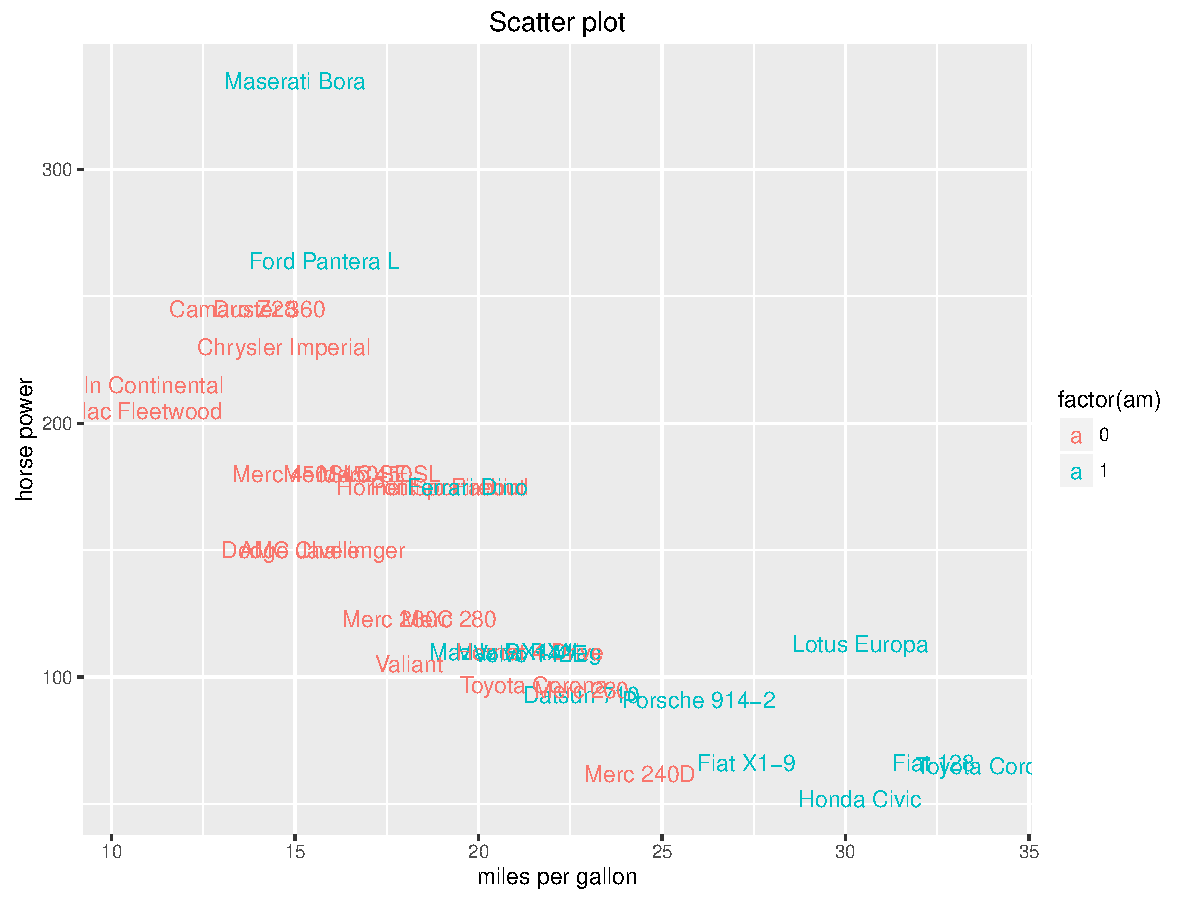
\includegraphics[width=.9\linewidth,height=.7\linewidth]{figure/your_xyplot3-1} 

}



\end{knitrout}

\end{frame}

%------------------------------------------------

\begin{frame}[fragile]
\frametitle{Text in scripts}

\begin{knitrout}\scriptsize
\definecolor{shadecolor}{rgb}{0.969, 0.969, 0.969}\color{fgcolor}\begin{kframe}
\begin{alltt}
\hlcom{# =====================================================}
\hlcom{# Stat133: Lab 2}
\hlcom{# Description: Basics of data frames}
\hlcom{# Data: Star Wars characters}
\hlcom{# =====================================================}

\hlcom{# load "readr}
\hlkwd{library}\hlstd{(}\hlstr{"readr"}\hlstd{)}

\hlcom{# read data using read_csv()}
\hlstd{sw} \hlkwb{<-} \hlkwd{read_csv}\hlstd{(}\hlstr{"~/stat133/datasets/starwarstoy.csv"}\hlstd{)}

\hlcom{# use str() to get information about the data frame structure}
\hlkwd{str}\hlstd{(sw)}

\hlcom{# use summary() to get some descriptive statistics}
\hlkwd{summary}\hlstd{(sw)}

\hlcom{# convert column 'gender' as a factor}
\hlstd{sw}\hlopt{$}\hlstd{gender} \hlkwb{<-} \hlkwd{factor}\hlstd{(sw}\hlopt{$}\hlstd{gender)}
\end{alltt}
\end{kframe}
\end{knitrout}

\end{frame}

%------------------------------------------------

\begin{frame}[fragile]
\frametitle{Text: names of files and directories}
\begin{center}
\ig[width=10cm]{images/dirfiles.png}
\end{center}
\end{frame}

%------------------------------------------------

\begin{frame}[fragile]
\frametitle{Wikipedia Table}

\begin{center}
\ig[width=6.5cm]{images/wikipedia_table.png}

\scalebox{.5}{\url{https://en.wikipedia.org/wiki/World_record_progression_1500_metres_freestyle
}}
\end{center}

\end{frame}

%------------------------------------------------

\begin{frame}[fragile]
\frametitle{Wikipedia Table}
\begin{center}
\ig[width=11cm]{images/wiki_swimming.png}
\end{center}
\end{frame}

%------------------------------------------------

\begin{frame}
\begin{center}
\Huge{\mdlit{Example: XML Data}}
\end{center}
\end{frame}

%------------------------------------------------

\begin{frame}[fragile]
\frametitle{Toy Data (XML format)}

\begin{knitrout}\footnotesize
\definecolor{shadecolor}{rgb}{0.969, 0.969, 0.969}\color{fgcolor}\begin{kframe}
\begin{alltt}
<subject>
  <name>
    <first>Luke</first>
    <last>Skywalker</last>
  </name>
  <gender>male</gender>
  <height>1.72</height>
</subject>
<subject>
  <name>
    <first>Leia</first>
    <last>Skywalker</last>
  </name>
  <gender>female</gender>
  <height>1.50</height>
</subject>
\end{alltt}
\end{kframe}
\end{knitrout}

\end{frame}

%------------------------------------------------

\begin{frame}
\frametitle{Extracting Data}

\bbi
  \item Sometimes we must extract the elements of interest from the text content
  \item The extraction is done by identifying the patterns where the values occur
\ei

\end{frame}

%------------------------------------------------

\begin{frame}
\frametitle{Extracting Data}

\bi
  \item A different example occurs when text itself makes up the data
  \item Speech
  \item Lyrics
  \item Email messages
  \item Abstract
  \item \textit{etc}
\ei

\end{frame}

%------------------------------------------------

\begin{frame}[fragile]
\frametitle{Example: Speech}

{\small Text of President Barack Obama's State of the Union address, as provided by the White House:

\begin{quotation}
Mr. Speaker, Mr. Vice President, members of Congress, distinguished guests and fellow Americans:

Last month, I went to Andrews Air Force Base and welcomed home some of our last troops to serve in Iraq. Together, we offered a final, proud salute to the colors under which more than a million of our fellow citizens fought-- and several thousand gave their lives.
\end{quotation}
}

\end{frame}

%------------------------------------------------

\begin{frame}
\frametitle{Example: Abstract}
\begin{center}
\ig[width=8cm]{images/pubmed_article.png}
\end{center}
\end{frame}

%------------------------------------------------

\begin{frame}
\begin{center}
\Huge{\mdlit{Example: Web Log}}
\end{center}
\end{frame}

%------------------------------------------------

\begin{frame}[fragile]
\frametitle{Web log example}

\begin{verbatim}
123.123.123.123 - - [26/Apr/2000:00:23:48 -0400] 
"GET /pics/wpaper.gif HTTP/1.0" 200 6248 
"http://www.jafsoft.com/asctortf/" 
"Mozilla/4.05 (Macintosh; I; PPC)"


123.123.123.123 - - [26/Apr/2000:00:23:47 -0400] 
"GET /asctortf/ HTTP/1.0" 200 8130 
"http://search.netscape.com/Computers/Data_Formats" 
"Mozilla/4.05 (Macintosh; I; PPC)"
\end{verbatim}

\end{frame}

%------------------------------------------------

\begin{frame}
\frametitle{Web log data}

\bi
  \item The information in the log has a lot of structure
  \item e.g. the date always appears in square brackets
  \item However, the information is not consistently separated by the same characters
  \item Nor is it placed consistently in the same columns in the file
\ei

\end{frame}

%------------------------------------------------

\begin{frame}[fragile]
\frametitle{Web log example}

Web log content structure:
\bigskip

{\small
\begin{verbatim}
ppp931.on.bellglobal.com
- -
[26/Apr/2000:00:16:12 -0400]
"GET /download/windows/asctab31.zip HTTP/1.0"
200
1540096
"http://www.htmlgoodies.com/downloads/freeware/15.html"
"Mozilla/4.7 [en]C-SYMPA  (Win95; U)"
\end{verbatim}
}

\end{frame}

%------------------------------------------------

\begin{frame}
\frametitle{Web log data}

\bi
  \item IP address: {\hilit \code{ppp931.on.bellglobal.com}}
  \item Username etc: {\hilit \code{"- -"}}
  \item Timestamp: {\hilit \code{"[26/Apr/2000:00:16:12 -0400]"}}
  \item Access request: \\ 
  {\hilit \code{"GET /download/windows/asctab31.zip HTTP/1.0"}}
  \item Result status code: {\hilit \code{"200"}}
  \item Bytes transferred: {\hilit \code{"1540096"}}
  \item Referrer URL: \\ {\hilit \footnotesize \code{"http://www.htmlgoodies.com/downloads/freeware/15.html"}}
  \item User Agent: {\hilit \code{"Mozilla/4.7 [en]C-SYMPA (Win95; U)"}}
\ei

\end{frame}

%------------------------------------------------

\begin{frame}
\frametitle{Spam Filtering}

\bb{Anatomy of an email message}
\bi
  \item Three parts:
  \bi
    \item header
    \item body
    \item attachments (optional)
  \ei
  \item Like regular mail, the header is the envelope and the body is the letter
  \item Plain text
\ei
\eb

\end{frame}

%------------------------------------------------

\begin{frame}
\frametitle{Spam Filtering}

\bb{Email header}
\bi
  \item date, sender, and subject
  \item message id
  \item who are the carbon-copy recipients
  \item return path
\ei
\eb

\end{frame}

%------------------------------------------------

\begin{frame}[fragile]
\frametitle{Example Email Header}

\begin{verbatim}
Date: Mon, 29 Jun 2015 22:16:19 -0800 (PST)
From: doe@email.edu
X-X-Sender: smith@email.net
To: Txxxx Uxxx <txxxx@uclink.berkeley.edu>
Subject: Re: prof: did you receive my hw?
In-Reply-To: <web-569552@calmail-st.berkeley.edu>
MIME-Version: 1.0
Content-Type: TEXT/PLAIN; charset=US-ASCII
Status: 0
X-Status: 
X-Keywords:
X-UID: 9079
\end{verbatim}

\end{frame}

%------------------------------------------------

\begin{frame}
\begin{center}
\Huge{\hilit{Motivation}}
\end{center}
\end{frame}

%------------------------------------------------

\begin{frame}
\frametitle{Motivation}

\bbi
  \item So far we have seen some basic and intermediate functions for handling and working with text in R
  \item These functions are very useful functions and they allows us to do many interesting things. 
  \item However, if we truly want to unleash the power of strings manipulation, we need to talk about \textit{regular expressions}.
\ei



\end{frame}

%------------------------------------------------

\begin{frame}[fragile]
\frametitle{Motivation}

\begin{knitrout}\footnotesize
\definecolor{shadecolor}{rgb}{0.969, 0.969, 0.969}\color{fgcolor}\begin{kframe}
\begin{verbatim}
##      name   gender   height   weight     born
## 1    Luke     male    1.72m     77gr    19BBY
## 2    Leia   Female    1.50m     49gr    19BBY
## 3   R2-D2     male    0.96m     32gr    33BBY
## 4   C-3PO     MALE    1.67m     75gr   112BBY
\end{verbatim}
\end{kframe}
\end{knitrout}

\pause
It is not uncommon to have datasets that need some cleaning and preprocessing

\end{frame}

%------------------------------------------------

\begin{frame}[fragile]
\frametitle{Motivation}

Some common tasks
\bi
  \item finding pieces of text or characters that meet a certain pattern
  \item extracting pieces of text in non-standard formats
  \item transforming text into a uniform format
  \item resolving inconsistencies
  \item substituting certain characters
  \item splitting a piece of text into various parts
\ei

\end{frame}

%------------------------------------------------

\begin{frame}
\begin{center}
\Huge{\hilit{Regular Expressions}}
\end{center}
\end{frame}

%------------------------------------------------

\begin{frame}
\frametitle{Regular Expressions}

\bbi
  \item A \textbf{regular expression} is a special text string for describing a certain amount of text.
  \item This ``certain amount of text'' receives the formal name of \textbf{pattern}. 
  \item A regular expression is a \textit{pattern that describes a set of strings}.
  \item It is common to abbreviate the term ``regular expression'' as \textbf{regex}
\ei

\end{frame}

%------------------------------------------------

\begin{frame}
\frametitle{Regular Expressions}

{\Large Simply put, working with regular expressions is nothing more than \textbf{pattern matching}}

\end{frame}

%------------------------------------------------

\begin{frame}
\frametitle{Regular Expressions}

\bi
  \item Regex patterns consist of a combination of alphanumeric characters as well as special characters.
  \bi
    \item e.g. \code{[a-zA-Z0-9\_.]*}
  \ei
  \item A regex pattern can be as simple as a single character
  \item But it can also be formed by several characters with a more complex structure
\ei

\end{frame}

%------------------------------------------------

\begin{frame}
\frametitle{About Regex}

\bi
  \item ``Regular Expressions'' is not a full programming language
  \item Regex have a special syntax and instructions that you must learn
  \item Regular expressions are supported in a variety of forms on almost every computing platform
  \item R has functions and packages designed to work with regular expressions
\ei

\end{frame}

%------------------------------------------------

\begin{frame}
\frametitle{Basic Concepts}

Regular expressions are constructed from 3 things:
\bbi
  \item \textbf{Literal characters} are matched only by the character itself
  \item A \textbf{character class} is matched by any single member of the specified class
  \item \textbf{Modifiers} operate on literal characters, character classes, or combinations of the two.
\ei

\end{frame}

%------------------------------------------------

\begin{frame}[fragile]
\frametitle{Literal Characters}

Consider the following text:
\begin{verbatim}
The quick brown fox jumps over the lazy dog
\end{verbatim}

\bigskip

A basic regex can be something as simple as {\hilit \code{fox}}. The characters \code{fox} match the word ``fox'' in the sentence above.

\end{frame}

%------------------------------------------------

\begin{frame}[fragile]
\frametitle{Special Characters}

Consider this other text:
\begin{verbatim}
One. Two. Three. And four* and Five!
\end{verbatim}

\bigskip

Not all characters are matched literally. There are some characters that have a special meaning in regular expressions: \textbf{.} or \textbf{*} are some of these special characters.

\end{frame}

%------------------------------------------------

\begin{frame}
\begin{center}
\Huge{\hilit{Special Characters}}
\end{center}
\end{frame}

%------------------------------------------------

\begin{frame}
\frametitle{Metacharacters}

\bi
  \item The simplest form of regular expressions are those that match a single character 
  \item Most characters, including all letters and digits, are regular expressions that match themselves
  \item For example, the pattern \code{"1"} matches the number 1
  \item The pattern \code{"blu"} matches the set of letters ``blu''.
  \item However, there are some special characters that don't match themselves
  \item These special characters are known as \textbf{metacharacters}.
\ei

\end{frame}

%------------------------------------------------

\begin{frame}[fragile]
\frametitle{Metacharacters}

The metacharacters in \textit{Extended Regular Expressions} are:
\begin{verbatim}
 .  \  |  (  )  [  {  $  *  +  ?
\end{verbatim}

\bigskip
To use a metacharacter symbol as a literal character, we need to \textbf{escape} them

\end{frame}

%------------------------------------------------

\begin{frame}[fragile]
\frametitle{}

\begin{center}
 \begin{tabular}{c l c}
  \multicolumn{3}{c}{\textbf{Metacharacters and how to escape them in R}} \\
 \hline
  Metacharacter & Literal meaning & Escape in R \\
  \hline
  \code{.} & the period or dot & \code{\textbackslash{\textbackslash{.}}} \\
  \code{\$} & the dollar sign & \code{\textbackslash{\textbackslash{\$}}} \\  
  \code{*} & the asterisk or star & \code{\textbackslash{\textbackslash{*}}} \\
  \code{+} & the plus sign & \code{\textbackslash{\textbackslash{+}}} \\
  \code{?} & the question mark & \code{\textbackslash{\textbackslash{?}}} \\
  \code{|} & the vertical bar or pipe symbol & \textbackslash{\textbackslash{\code{|}}} \\
  \code{\textbackslash{}} & the backslash & \textbackslash{\textbackslash{\textbackslash{\textbackslash{}}}} \\
  \code{\^} & the caret & \textbackslash{\textbackslash{\code{\^}}} \\
  \code{[} & the opening bracket & \textbackslash{\textbackslash{\code{[}}} \\
  \code{]} & the closing bracket & \textbackslash{\textbackslash{\code{]}}} \\
  \code{\{} & the opening brace & \textbackslash{\textbackslash{\code{\{}}} \\
  \code{\}} & the closing brace & \textbackslash{\textbackslash{\code{\}}}} \\
  \code{(} & the opening parenthesis & \textbackslash{\textbackslash{\code{(}}} \\
  \code{)} & the closing parenthesis & \textbackslash{\textbackslash{\code{)}}} \\
  \hline
 \end{tabular}
\end{center}

\end{frame}

%------------------------------------------------

\begin{frame}[fragile]
\frametitle{Character Classes}

\bi
  \item A \textit{character class} or \textit{character set} is a list of characters enclosed by square brackets \code{[ ]}
  \item Character sets are used to match \textbf{only one} of several characters.
  \item e.g. the regex character class \code{[aA]} matches any lower case letter \code{a} or any upper case letter \code{A}.
  \item character classes including the caret {\hilit \code{\^}} at the beginning of the list indicates that the regular expression matches any character \textbf{NOT} in the list
  \item A dash symbol {\hilit \code{-}} (not at the beginning) is used to indicate ranges: e.g. \code{[0-9]}
\ei

\end{frame}

%------------------------------------------------

\begin{frame}[fragile]
\frametitle{Character Classes}
\begin{knitrout}\footnotesize
\definecolor{shadecolor}{rgb}{0.969, 0.969, 0.969}\color{fgcolor}\begin{kframe}
\begin{alltt}
\hlcom{# some string}
\hlstd{transport} \hlkwb{<-} \hlkwd{c}\hlstd{(}\hlstr{"car"}\hlstd{,} \hlstr{"bike"}\hlstd{,} \hlstr{"plane"}\hlstd{,} \hlstr{"boat"}\hlstd{)}

\hlcom{# look for 'e' or 'i'}
\hlkwd{grep}\hlstd{(}\hlkwc{pattern} \hlstd{=} \hlstr{"[ei]"}\hlstd{, transport,} \hlkwc{value} \hlstd{=} \hlnum{TRUE}\hlstd{)}
\end{alltt}
\begin{verbatim}
## [1] "bike"  "plane"
\end{verbatim}
\end{kframe}
\end{knitrout}

\end{frame}

%------------------------------------------------

\begin{frame}[fragile]
\frametitle{Character Classes}

\begin{center}
 \begin{tabular}{c l}
  \multicolumn{2}{c}{\textbf{Some (Regex) Character Classes}} \\
 \hline
  Anchor & Description \\
  \hline
  \code{[aeiou]} & match any one lower case vowel \\  
  \code{[AEIOU]} & match any one upper case vowel \\
  \code{[0123456789]} & match any digit \\    
  \code{[0-9]} & match any digit (same as previous class) \\  
  \code{[a-z]} & match any lower case ASCII letter \\
  \code{[A-Z]} & match any upper case ASCII letter \\  
  \code{[a-zA-Z0-9]} & match any of the above classes \\
  \code{[\string^aeiou]} & match anything other than a lowercase vowel \\  
  \code{[\string^0-9]} & match anything other than a digit \\
  \hline
 \end{tabular}
\end{center}

\end{frame}

%------------------------------------------------

\begin{frame}[fragile]
\frametitle{POSIX Classes}

Closely related to the regex character classes we have what is known as \textit{POSIX character classes}. In R, POSIX character classes are represented with expressions inside double brackets \code{[[ ]]}.

\end{frame}

%------------------------------------------------

\begin{frame}[fragile]
\frametitle{POSIX Classes}

{\scriptsize 
\begin{center}
 \begin{tabular}{c l}
  \multicolumn{2}{c}{\textbf{POSIX Character Classes in R}} \\
 \hline
  Class & Description \\
  \hline
  \code{[[:lower:]]} & Lower-case letters \\  
  \code{[[:upper:]]} & Upper-case letters \\
  \code{[[:alpha:]]} & Alphabetic characters (\code{[[:lower:]]} and \code{[[:upper:]]}) \\
  \code{[[:digit:]]} & Digits: 0, 1, 2, 3, 4, 5, 6, 7, 8, 9 \\
  \code{[[:alnum:]]} & Alphanumeric characters (\code{[[:alpha:]]} and \code{[[:digit:]]}) \\  
  \code{[[:blank:]]} & Blank characters: space and tab \\  
  \code{[[:cntrl:]]} & Control characters \\  
  \code{[[:punct:]]} & Punctuation characters: ! " \# \% \& ' ( ) * + , - . / : ; \\
  \code{[[:space:]]} & Space characters: tab, newline, vertical tab, form feed, \\
  & carriage return, and space  \\  
  \code{[[:xdigit:]]} & Hexadecimal digits: 0-9 A B C D E F a b c d e f \\  
  \code{[[:print:]]} & Printable characters (\code{[[:alpha:]]}, \code{[[:punct:]]} and space) \\  
  \code{[[:graph:]]} & Graphical characters (\code{[[:alpha:]]} and \code{[[:punct:]]}) \\  
  \hline
 \end{tabular}
\end{center}
}

\end{frame}

%------------------------------------------------

\begin{frame}[fragile]
\frametitle{Special Sequences}

\textit{Sequences} define, no surprinsingly, sequences of characters which can match. 

\bigskip
There are shorthand versions (or anchors) for commonly used sequences

\end{frame}

%------------------------------------------------

\begin{frame}[fragile]
\frametitle{}

\begin{center}
 \begin{tabular}{c l}
  \multicolumn{2}{c}{\textbf{Anchor Sequences in R}} \\
 \hline
  Anchor & Description \\
  \hline
  \code{\textbackslash{\textbackslash{d}}} & match a digit character \\  
  \code{\textbackslash{\textbackslash{D}}} & match a non-digit character \\
  \code{\textbackslash{\textbackslash{s}}} & match a space character \\  
  \code{\textbackslash{\textbackslash{S}}} & match a non-space character \\
  \code{\textbackslash{\textbackslash{w}}} & match a word character \\  
  \code{\textbackslash{\textbackslash{W}}} & match a non-word character \\
  \code{\textbackslash{\textbackslash{b}}} & match a word boundary \\  
  \code{\textbackslash{\textbackslash{B}}} & match a non-(word boundary) \\
  \code{\textbackslash{\textbackslash{h}}} & match a horizontal space \\
  \code{\textbackslash{\textbackslash{H}}} & match a non-horizontal space \\
  \code{\textbackslash{\textbackslash{v}}} & match a vertical space \\
  \code{\textbackslash{\textbackslash{V}}} & match a non-vertical space \\
  \hline
 \end{tabular}
\end{center}

\end{frame}

%------------------------------------------------

\begin{frame}[fragile]
\frametitle{Quantifiers}

\bi
  \item Another important set of regex elements are the so-called \textit{quantifiers}. 
  \item These are used when we want to match a \textbf{certain number} of characters that meet certain criteria. 
  \item Quantifiers specify how many instances of a character, group, or character class must be present in the input for a match to be found. 
\ei

\end{frame}

%------------------------------------------------

\begin{frame}[fragile]
\frametitle{Quantifiers}

\begin{center}
 \begin{tabular}{c l}
 \hline
  Quantifier & Description \\
  \hline
  \code{?} & The preceding item is optional and will be \\
  & matched at most once \\  
  \code{*} & The preceding item will be matched zero \\
  & or more times \\
  \code{+} & The preceding item will be matched \\
  & one or more times \\
  \code{\{n\}} & The preceding item is matched exactly \code{n} times \\
  \code{\{n,\}} & The preceding item is matched \code{n} or more times \\
  \code{\{n,m\}} & The preceding item is matched at least \code{n} times, \\
  & but not more than \code{m} times \\
  \hline
 \end{tabular}
\end{center}

\end{frame}

%------------------------------------------------

\begin{frame}[fragile]
\frametitle{Positions}

\begin{center}
 \begin{tabular}{c l}
 \hline
  Character & Description \\
  \hline
  \code{\^} & matches the start of the string \\  
  \code{\$} & matches the end of the string \\
  \code{.} & matches any single character \\
  \code{|} & ``OR'' operator, matches patterns \\
  & on either side of the \code{|} \\
  \hline
 \end{tabular}
\end{center}

\end{frame}

%------------------------------------------------

\begin{frame}
\frametitle{Regex Tasks}

Common operations
\bi
  \item \textbf{Identify} a match to a pattern
  \item \textbf{Locate} a pattern match (positions)
  \item \textbf{Replace} a matched pattern
  \item \textbf{Extract} a matched pattern
\ei

\end{frame}

%------------------------------------------------

\begin{frame}
\begin{center}
\Huge{\hilit{Identify a Match}}
\end{center}
\end{frame}

%------------------------------------------------

\begin{frame}
\frametitle{Identify Matches}

Functions for identifying match to a pattern: 
\bbi
  \item \code{grep(..., value = FALSE)}
  \item \code{grepl()}
  \item \code{str\_detect()} (\code{"stringr"})
\ei

\end{frame}

%------------------------------------------------

\begin{frame}[fragile]
\frametitle{\code{grep(..., value = FALSE)}}

\begin{knitrout}\footnotesize
\definecolor{shadecolor}{rgb}{0.969, 0.969, 0.969}\color{fgcolor}\begin{kframe}
\begin{alltt}
\hlcom{# some text}
\hlstd{text} \hlkwb{<-} \hlkwd{c}\hlstd{(}\hlstr{"one word"}\hlstd{,} \hlstr{"a sentence"}\hlstd{,} \hlstr{"three two one"}\hlstd{)}

\hlcom{# pattern}
\hlstd{pat} \hlkwb{<-} \hlstr{"one"}

\hlcom{# default usage}
\hlkwd{grep}\hlstd{(pat, text)}
\end{alltt}
\begin{verbatim}
## [1] 1 3
\end{verbatim}
\end{kframe}
\end{knitrout}

\end{frame}

%------------------------------------------------

\begin{frame}[fragile]
\frametitle{\code{grepl()}}

\bbi
  \item \code{grepl()} is very similar to \code{grep()}
  \item The difference resides in that the output are not numeric indices, but logical
  \item You can think of \code{grepl()} as \code{grep}-\textit{logical}
\ei

\end{frame}

%------------------------------------------------

\begin{frame}[fragile]
\frametitle{\code{grepl()}}

\begin{knitrout}\footnotesize
\definecolor{shadecolor}{rgb}{0.969, 0.969, 0.969}\color{fgcolor}\begin{kframe}
\begin{alltt}
\hlcom{# some text}
\hlstd{text} \hlkwb{<-} \hlkwd{c}\hlstd{(}\hlstr{"one word"}\hlstd{,} \hlstr{"a sentence"}\hlstd{,} \hlstr{"three two one"}\hlstd{)}

\hlcom{# pattern}
\hlstd{pat} \hlkwb{<-} \hlstr{"one"}

\hlcom{# default usage}
\hlkwd{grepl}\hlstd{(pat, text)}
\end{alltt}
\begin{verbatim}
## [1]  TRUE FALSE  TRUE
\end{verbatim}
\end{kframe}
\end{knitrout}

\end{frame}

%------------------------------------------------

\begin{frame}[fragile]
\frametitle{\code{str\_detect()} in \code{"stringr"}}

\begin{knitrout}\footnotesize
\definecolor{shadecolor}{rgb}{0.969, 0.969, 0.969}\color{fgcolor}\begin{kframe}
\begin{alltt}
\hlcom{# some text}
\hlstd{text} \hlkwb{<-} \hlkwd{c}\hlstd{(}\hlstr{"one word"}\hlstd{,} \hlstr{"a sentence"}\hlstd{,} \hlstr{"three two one"}\hlstd{)}

\hlcom{# pattern}
\hlstd{pat} \hlkwb{<-} \hlstr{"one"}

\hlcom{# default usage}
\hlkwd{str_detect}\hlstd{(text, pat)}
\end{alltt}
\begin{verbatim}
## [1]  TRUE FALSE  TRUE
\end{verbatim}
\end{kframe}
\end{knitrout}

\end{frame}

%------------------------------------------------

\begin{frame}
\begin{center}
\Huge{\hilit{Locate a Match}}
\end{center}
\end{frame}

%------------------------------------------------

\begin{frame}
\frametitle{Locate Matches}

Functions for locating match to a pattern: 
\bbi
  \item \code{regexpr()}
  \item \code{gregexpr()}
  \item \code{str\_locate()} (\code{"stringr"})
  \item \code{str\_locate\_all()} (\code{"stringr"})
\ei

\end{frame}

%------------------------------------------------

\begin{frame}[fragile]
\frametitle{\code{regexpr()}}

\bi
  \item \code{regexpr()} is used to find exactly where the pattern is found in a given string
  \item it tells us which elements of the text vector actually contain the regex pattern, and
 \item identifies the position of the substring that is matched by the regex pattern
\ei

\end{frame}

%------------------------------------------------

\begin{frame}[fragile]
\frametitle{\code{regexpr()}}

\begin{knitrout}\footnotesize
\definecolor{shadecolor}{rgb}{0.969, 0.969, 0.969}\color{fgcolor}\begin{kframe}
\begin{alltt}
\hlcom{# some text}
\hlstd{text} \hlkwb{<-} \hlkwd{c}\hlstd{(}\hlstr{"one word"}\hlstd{,} \hlstr{"a sentence"}\hlstd{,} \hlstr{"three two one"}\hlstd{)}

\hlcom{# default usage}
\hlkwd{regexpr}\hlstd{(}\hlkwc{pattern} \hlstd{=} \hlstr{"one"}\hlstd{, text)}
\end{alltt}
\begin{verbatim}
## [1]  1 -1 11
## attr(,"match.length")
## [1]  3 -1  3
## attr(,"useBytes")
## [1] TRUE
\end{verbatim}
\end{kframe}
\end{knitrout}

\end{frame}

%------------------------------------------------

\begin{frame}[fragile]
\frametitle{\code{gregexpr()}}

\bi
  \item \code{gregexpr()} does practically the same thing as \code{regexpr()}
  \item identifies where a pattern is within a string vector, by searching each element separately
  \item The only difference is that \code{gregexpr()} has an output in the form of a list
\ei

\end{frame}

%------------------------------------------------

\begin{frame}[fragile]
\frametitle{\code{gregexpr()}}

\begin{knitrout}\tiny
\definecolor{shadecolor}{rgb}{0.969, 0.969, 0.969}\color{fgcolor}\begin{kframe}
\begin{alltt}
\hlcom{# some text}
\hlstd{text} \hlkwb{<-} \hlkwd{c}\hlstd{(}\hlstr{"one word"}\hlstd{,} \hlstr{"a sentence"}\hlstd{,} \hlstr{"three two one"}\hlstd{)}

\hlcom{# default usage}
\hlkwd{gregexpr}\hlstd{(}\hlkwc{pattern} \hlstd{=} \hlstr{"one"}\hlstd{, text)}
\end{alltt}
\begin{verbatim}
## [[1]]
## [1] 1
## attr(,"match.length")
## [1] 3
## attr(,"useBytes")
## [1] TRUE
## 
## [[2]]
## [1] -1
## attr(,"match.length")
## [1] -1
## attr(,"useBytes")
## [1] TRUE
## 
## [[3]]
## [1] 11
## attr(,"match.length")
## [1] 3
## attr(,"useBytes")
## [1] TRUE
\end{verbatim}
\end{kframe}
\end{knitrout}

\end{frame}

%------------------------------------------------

\begin{frame}[fragile]
\frametitle{\code{str\_locate()} in \code{"stringr"}}

\bi
  \item \code{str\_locate()} locates the position of the first occurrence of a pattern in a string
  \item it tells us which elements of the text vector actually contain the regex pattern, and
 \item identifies the position of the substring that is matched by the regex pattern
\ei

\end{frame}

%------------------------------------------------

\begin{frame}[fragile]
\frametitle{\code{str\_locate()} in \code{"stringr"}}

\begin{knitrout}\footnotesize
\definecolor{shadecolor}{rgb}{0.969, 0.969, 0.969}\color{fgcolor}\begin{kframe}
\begin{alltt}
\hlcom{# some text}
\hlstd{text} \hlkwb{<-} \hlkwd{c}\hlstd{(}\hlstr{"one word"}\hlstd{,} \hlstr{"a sentence"}\hlstd{,} \hlstr{"three two one"}\hlstd{)}

\hlcom{# default usage}
\hlkwd{str_locate}\hlstd{(text,} \hlkwc{pattern} \hlstd{=} \hlstr{"one"}\hlstd{)}
\end{alltt}
\begin{verbatim}
##      start end
## [1,]     1   3
## [2,]    NA  NA
## [3,]    11  13
\end{verbatim}
\end{kframe}
\end{knitrout}

\end{frame}

%------------------------------------------------

\begin{frame}[fragile]
\frametitle{\code{str\_locate\_all()} in \code{"stringr"}}

\bi
  \item \code{str\_locate\_all()} locates the position of ALL the occurrences of a pattern in a string
  \item it tells us which elements of the text vector actually contain the regex pattern, and
 \item the output is in the form of a list with as many elements as the number of elements in the examined vector
\ei

\end{frame}

%------------------------------------------------

\begin{frame}[fragile]
\frametitle{\code{str\_locate\_all()} in \code{"stringr"}}

\begin{knitrout}\footnotesize
\definecolor{shadecolor}{rgb}{0.969, 0.969, 0.969}\color{fgcolor}\begin{kframe}
\begin{alltt}
\hlcom{# some text}
\hlstd{text} \hlkwb{<-} \hlkwd{c}\hlstd{(}\hlstr{"one word"}\hlstd{,} \hlstr{"a sentence"}\hlstd{,} \hlstr{"one three two one"}\hlstd{)}

\hlcom{# default usage}
\hlkwd{str_locate_all}\hlstd{(text,} \hlkwc{pattern} \hlstd{=} \hlstr{"one"}\hlstd{)}
\end{alltt}
\begin{verbatim}
## [[1]]
##      start end
## [1,]     1   3
## 
## [[2]]
##      start end
## 
## [[3]]
##      start end
## [1,]     1   3
## [2,]    15  17
\end{verbatim}
\end{kframe}
\end{knitrout}

\end{frame}

%------------------------------------------------

\begin{frame}
\begin{center}
\Huge{\hilit{Extract a Match}}
\end{center}
\end{frame}

%------------------------------------------------

\begin{frame}
\frametitle{Extract Matches}

Functions for extracting positions of matched pattern: 
\bbi
  \item \code{grep(..., value = TRUE)}
  \item \code{str\_extract()} (\code{"stringr"})
  \item \code{str\_extract\_all()} (\code{"stringr"})
\ei

\end{frame}

%------------------------------------------------

\begin{frame}[fragile]
\frametitle{Extraction with \code{grep(..., value = TRUE)}}

\bi
  \item {\hilit \code{grep(..., value = TRUE)}} allows us to do basic extraction
  \item Actually, it will extract the entire element that matches the pattern
  \item Sometimes this is not exactly what we want to do (it's better to use functions of \code{"stringr"})
\ei

\end{frame}

%------------------------------------------------

\begin{frame}[fragile]
\frametitle{\code{grep(..., value = TRUE)}}

\begin{knitrout}\footnotesize
\definecolor{shadecolor}{rgb}{0.969, 0.969, 0.969}\color{fgcolor}\begin{kframe}
\begin{alltt}
\hlcom{# some text}
\hlstd{text} \hlkwb{<-} \hlkwd{c}\hlstd{(}\hlstr{"one word"}\hlstd{,} \hlstr{"a sentence"}\hlstd{,} \hlstr{"one three two one"}\hlstd{)}

\hlcom{# extract first one}
\hlkwd{grep}\hlstd{(}\hlkwc{pattern} \hlstd{=} \hlstr{"one"}\hlstd{, text,} \hlkwc{value} \hlstd{=} \hlnum{TRUE}\hlstd{)}
\end{alltt}
\begin{verbatim}
## [1] "one word"          "one three two one"
\end{verbatim}
\end{kframe}
\end{knitrout}

\end{frame}

%------------------------------------------------

\begin{frame}[fragile]
\frametitle{Pattern extraction with \code{str\_extract()}}

\bbi
  \item {\hilit \code{str\_extract()}} extracts the first occurrence of the matched pattern
  \item It will only extract the matched pattern
  \item If no pattern is matched, then a missing value is returned
\ei

\end{frame}

%------------------------------------------------

\begin{frame}[fragile]
\frametitle{\code{str\_extract()} in \code{"stringr"}}

\begin{knitrout}\footnotesize
\definecolor{shadecolor}{rgb}{0.969, 0.969, 0.969}\color{fgcolor}\begin{kframe}
\begin{alltt}
\hlcom{# some text}
\hlstd{text} \hlkwb{<-} \hlkwd{c}\hlstd{(}\hlstr{"one word"}\hlstd{,} \hlstr{"a sentence"}\hlstd{,} \hlstr{"one three two one"}\hlstd{)}

\hlcom{# extract first one}
\hlkwd{str_extract}\hlstd{(text,} \hlkwc{pattern} \hlstd{=} \hlstr{"one"}\hlstd{)}
\end{alltt}
\begin{verbatim}
## [1] "one" NA    "one"
\end{verbatim}
\end{kframe}
\end{knitrout}

\end{frame}

%------------------------------------------------

\begin{frame}[fragile]
\frametitle{Pattern extraction with \code{str\_extract\_all()}}

\bbi
  \item {\hilit \code{str\_extract\_all()}} extracts ALL the occurrences of the matched pattern
  \item It will only extract the matched pattern
  \item If no pattern is matched, then a character vector of length zero is returned
  \item the output is in list format
\ei

\end{frame}

%------------------------------------------------

\begin{frame}[fragile]
\frametitle{\code{str\_extract\_all()} in \code{"stringr"}}

\begin{knitrout}\footnotesize
\definecolor{shadecolor}{rgb}{0.969, 0.969, 0.969}\color{fgcolor}\begin{kframe}
\begin{alltt}
\hlcom{# some text}
\hlstd{text} \hlkwb{<-} \hlkwd{c}\hlstd{(}\hlstr{"one word"}\hlstd{,} \hlstr{"a sentence"}\hlstd{,} \hlstr{"one three two one"}\hlstd{)}

\hlcom{# extract all 'one's}
\hlkwd{str_extract_all}\hlstd{(text,} \hlkwc{pattern} \hlstd{=} \hlstr{"one"}\hlstd{)}
\end{alltt}
\begin{verbatim}
## [[1]]
## [1] "one"
## 
## [[2]]
## character(0)
## 
## [[3]]
## [1] "one" "one"
\end{verbatim}
\end{kframe}
\end{knitrout}

\end{frame}

%------------------------------------------------

\begin{frame}
\begin{center}
\Huge{\hilit{Replace a Match}}
\end{center}
\end{frame}

%------------------------------------------------

\begin{frame}
\frametitle{Replace Matches}

Functions for replacing a matched pattern: 
\bbi
  \item \code{sub()}
  \item \code{gsub()}
  \item \code{str\_replace()} (\code{"stringr"})
  \item \code{str\_replace\_all()} (\code{"stringr"})
\ei

\end{frame}

%------------------------------------------------

\begin{frame}
\frametitle{Replace first occurrence with \code{sub()}}

About {\hilit \code{sub()}}
\bbi
  \item \code{sub()} replaces the \textbf{first} occurrence of a pattern in a given text
  \item if there is more than one occurrence of the pattern in each element of a string vector, only the first one will be replaced.
\ei

\end{frame}

%------------------------------------------------

\begin{frame}[fragile]
\frametitle{Replacing with \code{sub()}}

\begin{knitrout}\scriptsize
\definecolor{shadecolor}{rgb}{0.969, 0.969, 0.969}\color{fgcolor}\begin{kframe}
\begin{alltt}
\hlcom{# string}
\hlstd{Rstring} \hlkwb{<-} \hlkwd{c}\hlstd{(}\hlstr{"The R Foundation"}\hlstd{,}
            \hlstr{"for Statistical Computing"}\hlstd{,}
            \hlstr{"R is FREE software"}\hlstd{,}
            \hlstr{"R is a collaborative project"}\hlstd{)}

\hlcom{# substitute first 'R' with 'RR'}
\hlkwd{sub}\hlstd{(}\hlstr{"R"}\hlstd{,} \hlstr{"RR"}\hlstd{, Rstring)}
\end{alltt}
\begin{verbatim}
## [1] "The RR Foundation"             "for Statistical Computing"    
## [3] "RR is FREE software"           "RR is a collaborative project"
\end{verbatim}
\end{kframe}
\end{knitrout}

\end{frame}

%------------------------------------------------

\begin{frame}
\frametitle{Replace all occurrences with \code{gsub()}}

To replace not only the first pattern occurrence, but \textbf{all} of the occurrences we should use {\hilit \code{gsub()}} (think of it as \textit{general} substitution)

\end{frame}

%------------------------------------------------

\begin{frame}[fragile]
\frametitle{Replacing with \code{gsub()}}

\begin{knitrout}\scriptsize
\definecolor{shadecolor}{rgb}{0.969, 0.969, 0.969}\color{fgcolor}\begin{kframe}
\begin{alltt}
\hlcom{# string}
\hlstd{Rstring} \hlkwb{<-} \hlkwd{c}\hlstd{(}\hlstr{"The R Foundation"}\hlstd{,}
            \hlstr{"for Statistical Computing"}\hlstd{,}
            \hlstr{"R is FREE software"}\hlstd{,}
            \hlstr{"R is a collaborative project"}\hlstd{)}

\hlcom{# substitute all 'R' with 'RR'}
\hlkwd{gsub}\hlstd{(}\hlstr{"R"}\hlstd{,} \hlstr{"RR"}\hlstd{, Rstring)}
\end{alltt}
\begin{verbatim}
## [1] "The RR Foundation"             "for Statistical Computing"    
## [3] "RR is FRREE software"          "RR is a collaborative project"
\end{verbatim}
\end{kframe}
\end{knitrout}

\end{frame}

%------------------------------------------------

\begin{frame}[fragile]
\frametitle{Replacing with \code{str\_replace()}}

\begin{knitrout}\scriptsize
\definecolor{shadecolor}{rgb}{0.969, 0.969, 0.969}\color{fgcolor}\begin{kframe}
\begin{alltt}
\hlcom{# string}
\hlstd{Rstring} \hlkwb{<-} \hlkwd{c}\hlstd{(}\hlstr{"The R Foundation"}\hlstd{,}
            \hlstr{"for Statistical Computing"}\hlstd{,}
            \hlstr{"R is FREE software"}\hlstd{,}
            \hlstr{"R is a collaborative project"}\hlstd{)}

\hlcom{# substitute first 'R' with 'RR'}
\hlkwd{str_replace}\hlstd{(Rstring,} \hlstr{"R"}\hlstd{,} \hlstr{"RR"}\hlstd{)}
\end{alltt}
\begin{verbatim}
## [1] "The RR Foundation"             "for Statistical Computing"    
## [3] "RR is FREE software"           "RR is a collaborative project"
\end{verbatim}
\end{kframe}
\end{knitrout}

\end{frame}

%------------------------------------------------

\begin{frame}[fragile]
\frametitle{Replacing with \code{str\_replace\_all()}}

\begin{knitrout}\scriptsize
\definecolor{shadecolor}{rgb}{0.969, 0.969, 0.969}\color{fgcolor}\begin{kframe}
\begin{alltt}
\hlcom{# string}
\hlstd{Rstring} \hlkwb{<-} \hlkwd{c}\hlstd{(}\hlstr{"The R Foundation"}\hlstd{,}
            \hlstr{"for Statistical Computing"}\hlstd{,}
            \hlstr{"R is FREE software"}\hlstd{,}
            \hlstr{"R is a collaborative project"}\hlstd{)}

\hlcom{# substitute first 'R' with 'RR'}
\hlkwd{str_replace_all}\hlstd{(Rstring,} \hlstr{"R"}\hlstd{,} \hlstr{"RR"}\hlstd{)}
\end{alltt}
\begin{verbatim}
## [1] "The RR Foundation"             "for Statistical Computing"    
## [3] "RR is FRREE software"          "RR is a collaborative project"
\end{verbatim}
\end{kframe}
\end{knitrout}

\end{frame}

%------------------------------------------------

\begin{frame}
\begin{center}
\Huge{\hilit{Split a string}}
\end{center}
\end{frame}

%------------------------------------------------

\begin{frame}
\frametitle{Split a string}

Another common task is \textit{splitting} a string based on a pattern. The idea is to split the elements of a character vector into substrings according to regex matches.

\end{frame}

%------------------------------------------------

\begin{frame}
\frametitle{Split a string}

Functions for extracting positions of matched pattern: 
\bbi
  \item \code{strsplit()}
  \item \code{str\_split()} (\code{"stringr"})
\ei

\end{frame}

%------------------------------------------------

\begin{frame}[fragile]
\frametitle{Split a string}

\begin{knitrout}\footnotesize
\definecolor{shadecolor}{rgb}{0.969, 0.969, 0.969}\color{fgcolor}\begin{kframe}
\begin{alltt}
\hlcom{# a sentence}
\hlstd{sentence} \hlkwb{<-} \hlkwd{c}\hlstd{(}\hlstr{"The quick brown fox"}\hlstd{)}

\hlcom{# split into words}
\hlkwd{strsplit}\hlstd{(sentence,} \hlstr{" "}\hlstd{)}
\end{alltt}
\begin{verbatim}
## [[1]]
## [1] "The"   "quick" "brown" "fox"
\end{verbatim}
\end{kframe}
\end{knitrout}

\end{frame}

%------------------------------------------------

\begin{frame}[fragile]
\frametitle{Split a string}

\begin{knitrout}\footnotesize
\definecolor{shadecolor}{rgb}{0.969, 0.969, 0.969}\color{fgcolor}\begin{kframe}
\begin{alltt}
\hlcom{# telephone numbers}
\hlstd{tels} \hlkwb{<-} \hlkwd{c}\hlstd{(}\hlstr{"510-548-2238"}\hlstd{,} \hlstr{"707-231-2440"}\hlstd{,} \hlstr{"650-752-1300"}\hlstd{)}

\hlcom{# split each number into its portions}
\hlkwd{strsplit}\hlstd{(tels,} \hlstr{"-"}\hlstd{)}
\end{alltt}
\begin{verbatim}
## [[1]]
## [1] "510"  "548"  "2238"
## 
## [[2]]
## [1] "707"  "231"  "2440"
## 
## [[3]]
## [1] "650"  "752"  "1300"
\end{verbatim}
\end{kframe}
\end{knitrout}

\end{frame}

%------------------------------------------------

\begin{frame}[fragile]
\frametitle{Split a string}

\begin{knitrout}\footnotesize
\definecolor{shadecolor}{rgb}{0.969, 0.969, 0.969}\color{fgcolor}\begin{kframe}
\begin{alltt}
\hlcom{# telephone numbers}
\hlstd{tels} \hlkwb{<-} \hlkwd{c}\hlstd{(}\hlstr{"510-548-2238"}\hlstd{,} \hlstr{"707-231-2440"}\hlstd{,} \hlstr{"650-752-1300"}\hlstd{)}

\hlcom{# split each number into its portions}
\hlkwd{str_split}\hlstd{(tels,} \hlstr{"-"}\hlstd{)}
\end{alltt}
\begin{verbatim}
## [[1]]
## [1] "510"  "548"  "2238"
## 
## [[2]]
## [1] "707"  "231"  "2440"
## 
## [[3]]
## [1] "650"  "752"  "1300"
\end{verbatim}
\end{kframe}
\end{knitrout}

\end{frame}


%------------------------------------------------

\end{document}
